% Graphic for TeX using PGF
% Title: /home/alex/WualaDrive/myfiles/Uni/4 Semester/Algorithmen/Skript/algorithmen/Diagramm17.dia
% Creator: Dia v0.97.1
% CreationDate: Tue May 11 15:48:36 2010
% For: alex
% \usepackage{tikz}
% The following commands are not supported in PSTricks at present
% We define them conditionally, so when they are implemented,
% this pgf file will use them.
\ifx\du\undefined
  \newlength{\du}
\fi
\setlength{\du}{15\unitlength}
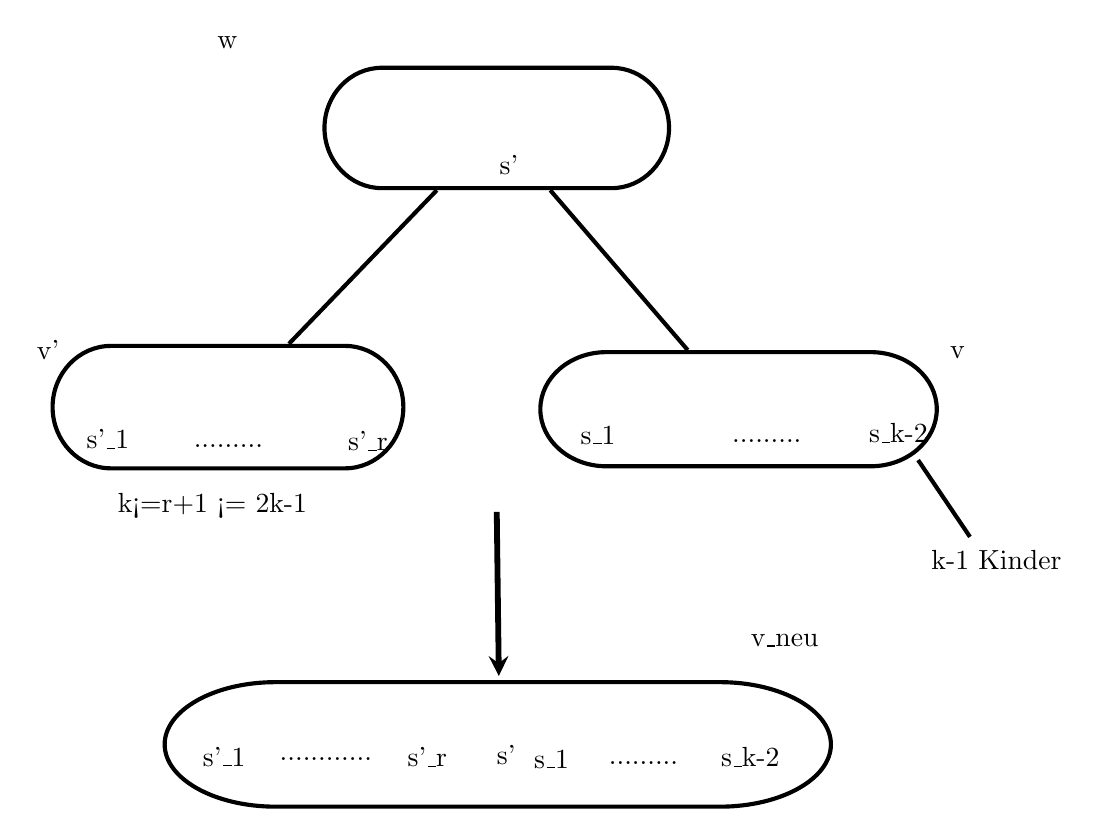
\begin{tikzpicture}
\pgftransformxscale{1.000000}
\pgftransformyscale{-1.000000}
\definecolor{dialinecolor}{rgb}{0.000000, 0.000000, 0.000000}
\pgfsetstrokecolor{dialinecolor}
\definecolor{dialinecolor}{rgb}{1.000000, 1.000000, 1.000000}
\pgfsetfillcolor{dialinecolor}
\pgfsetlinewidth{0.100000\du}
\pgfsetdash{}{0pt}
\pgfsetdash{}{0pt}
\pgfsetbuttcap
\pgfsetmiterjoin
\pgfsetlinewidth{0.100000\du}
\pgfsetbuttcap
\pgfsetmiterjoin
\pgfsetdash{}{0pt}
\definecolor{dialinecolor}{rgb}{1.000000, 1.000000, 1.000000}
\pgfsetfillcolor{dialinecolor}
\pgfpathmoveto{\pgfpoint{12.533333\du}{6.350000\du}}
\pgfpathlineto{\pgfpoint{18.066667\du}{6.350000\du}}
\pgfpathcurveto{\pgfpoint{18.830661\du}{6.350000\du}}{\pgfpoint{19.450000\du}{6.999187\du}}{\pgfpoint{19.450000\du}{7.800000\du}}
\pgfpathcurveto{\pgfpoint{19.450000\du}{8.600813\du}}{\pgfpoint{18.830661\du}{9.250000\du}}{\pgfpoint{18.066667\du}{9.250000\du}}
\pgfpathlineto{\pgfpoint{12.533333\du}{9.250000\du}}
\pgfpathcurveto{\pgfpoint{11.769339\du}{9.250000\du}}{\pgfpoint{11.150000\du}{8.600813\du}}{\pgfpoint{11.150000\du}{7.800000\du}}
\pgfpathcurveto{\pgfpoint{11.150000\du}{6.999187\du}}{\pgfpoint{11.769339\du}{6.350000\du}}{\pgfpoint{12.533333\du}{6.350000\du}}
\pgfusepath{fill}
\definecolor{dialinecolor}{rgb}{0.000000, 0.000000, 0.000000}
\pgfsetstrokecolor{dialinecolor}
\pgfpathmoveto{\pgfpoint{12.533333\du}{6.350000\du}}
\pgfpathlineto{\pgfpoint{18.066667\du}{6.350000\du}}
\pgfpathcurveto{\pgfpoint{18.830661\du}{6.350000\du}}{\pgfpoint{19.450000\du}{6.999187\du}}{\pgfpoint{19.450000\du}{7.800000\du}}
\pgfpathcurveto{\pgfpoint{19.450000\du}{8.600813\du}}{\pgfpoint{18.830661\du}{9.250000\du}}{\pgfpoint{18.066667\du}{9.250000\du}}
\pgfpathlineto{\pgfpoint{12.533333\du}{9.250000\du}}
\pgfpathcurveto{\pgfpoint{11.769339\du}{9.250000\du}}{\pgfpoint{11.150000\du}{8.600813\du}}{\pgfpoint{11.150000\du}{7.800000\du}}
\pgfpathcurveto{\pgfpoint{11.150000\du}{6.999187\du}}{\pgfpoint{11.769339\du}{6.350000\du}}{\pgfpoint{12.533333\du}{6.350000\du}}
\pgfusepath{stroke}
% setfont left to latex
\definecolor{dialinecolor}{rgb}{0.000000, 0.000000, 0.000000}
\pgfsetstrokecolor{dialinecolor}
\node at (15.300000\du,8.000000\du){};
\pgfsetlinewidth{0.100000\du}
\pgfsetdash{}{0pt}
\pgfsetdash{}{0pt}
\pgfsetbuttcap
\pgfsetmiterjoin
\pgfsetlinewidth{0.100000\du}
\pgfsetbuttcap
\pgfsetmiterjoin
\pgfsetdash{}{0pt}
\definecolor{dialinecolor}{rgb}{1.000000, 1.000000, 1.000000}
\pgfsetfillcolor{dialinecolor}
\pgfpathmoveto{\pgfpoint{6.008333\du}{13.050000\du}}
\pgfpathlineto{\pgfpoint{11.641667\du}{13.050000\du}}
\pgfpathcurveto{\pgfpoint{12.419468\du}{13.050000\du}}{\pgfpoint{13.050000\du}{13.710380\du}}{\pgfpoint{13.050000\du}{14.525000\du}}
\pgfpathcurveto{\pgfpoint{13.050000\du}{15.339620\du}}{\pgfpoint{12.419468\du}{16.000000\du}}{\pgfpoint{11.641667\du}{16.000000\du}}
\pgfpathlineto{\pgfpoint{6.008333\du}{16.000000\du}}
\pgfpathcurveto{\pgfpoint{5.230532\du}{16.000000\du}}{\pgfpoint{4.600000\du}{15.339620\du}}{\pgfpoint{4.600000\du}{14.525000\du}}
\pgfpathcurveto{\pgfpoint{4.600000\du}{13.710380\du}}{\pgfpoint{5.230532\du}{13.050000\du}}{\pgfpoint{6.008333\du}{13.050000\du}}
\pgfusepath{fill}
\definecolor{dialinecolor}{rgb}{0.000000, 0.000000, 0.000000}
\pgfsetstrokecolor{dialinecolor}
\pgfpathmoveto{\pgfpoint{6.008333\du}{13.050000\du}}
\pgfpathlineto{\pgfpoint{11.641667\du}{13.050000\du}}
\pgfpathcurveto{\pgfpoint{12.419468\du}{13.050000\du}}{\pgfpoint{13.050000\du}{13.710380\du}}{\pgfpoint{13.050000\du}{14.525000\du}}
\pgfpathcurveto{\pgfpoint{13.050000\du}{15.339620\du}}{\pgfpoint{12.419468\du}{16.000000\du}}{\pgfpoint{11.641667\du}{16.000000\du}}
\pgfpathlineto{\pgfpoint{6.008333\du}{16.000000\du}}
\pgfpathcurveto{\pgfpoint{5.230532\du}{16.000000\du}}{\pgfpoint{4.600000\du}{15.339620\du}}{\pgfpoint{4.600000\du}{14.525000\du}}
\pgfpathcurveto{\pgfpoint{4.600000\du}{13.710380\du}}{\pgfpoint{5.230532\du}{13.050000\du}}{\pgfpoint{6.008333\du}{13.050000\du}}
\pgfusepath{stroke}
% setfont left to latex
\definecolor{dialinecolor}{rgb}{0.000000, 0.000000, 0.000000}
\pgfsetstrokecolor{dialinecolor}
\node at (8.825000\du,14.725000\du){};
\pgfsetlinewidth{0.100000\du}
\pgfsetdash{}{0pt}
\pgfsetdash{}{0pt}
\pgfsetbuttcap
\pgfsetmiterjoin
\pgfsetlinewidth{0.100000\du}
\pgfsetbuttcap
\pgfsetmiterjoin
\pgfsetdash{}{0pt}
\definecolor{dialinecolor}{rgb}{1.000000, 1.000000, 1.000000}
\pgfsetfillcolor{dialinecolor}
\pgfpathmoveto{\pgfpoint{17.941667\du}{13.200000\du}}
\pgfpathlineto{\pgfpoint{24.308333\du}{13.200000\du}}
\pgfpathcurveto{\pgfpoint{25.187387\du}{13.200000\du}}{\pgfpoint{25.900000\du}{13.815608\du}}{\pgfpoint{25.900000\du}{14.575000\du}}
\pgfpathcurveto{\pgfpoint{25.900000\du}{15.334392\du}}{\pgfpoint{25.187387\du}{15.950000\du}}{\pgfpoint{24.308333\du}{15.950000\du}}
\pgfpathlineto{\pgfpoint{17.941667\du}{15.950000\du}}
\pgfpathcurveto{\pgfpoint{17.062613\du}{15.950000\du}}{\pgfpoint{16.350000\du}{15.334392\du}}{\pgfpoint{16.350000\du}{14.575000\du}}
\pgfpathcurveto{\pgfpoint{16.350000\du}{13.815608\du}}{\pgfpoint{17.062613\du}{13.200000\du}}{\pgfpoint{17.941667\du}{13.200000\du}}
\pgfusepath{fill}
\definecolor{dialinecolor}{rgb}{0.000000, 0.000000, 0.000000}
\pgfsetstrokecolor{dialinecolor}
\pgfpathmoveto{\pgfpoint{17.941667\du}{13.200000\du}}
\pgfpathlineto{\pgfpoint{24.308333\du}{13.200000\du}}
\pgfpathcurveto{\pgfpoint{25.187387\du}{13.200000\du}}{\pgfpoint{25.900000\du}{13.815608\du}}{\pgfpoint{25.900000\du}{14.575000\du}}
\pgfpathcurveto{\pgfpoint{25.900000\du}{15.334392\du}}{\pgfpoint{25.187387\du}{15.950000\du}}{\pgfpoint{24.308333\du}{15.950000\du}}
\pgfpathlineto{\pgfpoint{17.941667\du}{15.950000\du}}
\pgfpathcurveto{\pgfpoint{17.062613\du}{15.950000\du}}{\pgfpoint{16.350000\du}{15.334392\du}}{\pgfpoint{16.350000\du}{14.575000\du}}
\pgfpathcurveto{\pgfpoint{16.350000\du}{13.815608\du}}{\pgfpoint{17.062613\du}{13.200000\du}}{\pgfpoint{17.941667\du}{13.200000\du}}
\pgfusepath{stroke}
% setfont left to latex
\definecolor{dialinecolor}{rgb}{0.000000, 0.000000, 0.000000}
\pgfsetstrokecolor{dialinecolor}
\node at (21.125000\du,14.775000\du){};
% setfont left to latex
\definecolor{dialinecolor}{rgb}{0.000000, 0.000000, 0.000000}
\pgfsetstrokecolor{dialinecolor}
\node[anchor=west] at (8.300000\du,5.750000\du){w};
% setfont left to latex
\definecolor{dialinecolor}{rgb}{0.000000, 0.000000, 0.000000}
\pgfsetstrokecolor{dialinecolor}
\node[anchor=west] at (3.950000\du,13.150000\du){v'};
% setfont left to latex
\definecolor{dialinecolor}{rgb}{0.000000, 0.000000, 0.000000}
\pgfsetstrokecolor{dialinecolor}
\node[anchor=west] at (25.950000\du,13.200000\du){v};
\pgfsetlinewidth{0.100000\du}
\pgfsetdash{}{0pt}
\pgfsetdash{}{0pt}
\pgfsetbuttcap
{
\definecolor{dialinecolor}{rgb}{0.000000, 0.000000, 0.000000}
\pgfsetfillcolor{dialinecolor}
% was here!!!
\definecolor{dialinecolor}{rgb}{0.000000, 0.000000, 0.000000}
\pgfsetstrokecolor{dialinecolor}
\draw (13.856720\du,9.299005\du)--(10.292783\du,13.000546\du);
}
\pgfsetlinewidth{0.100000\du}
\pgfsetdash{}{0pt}
\pgfsetdash{}{0pt}
\pgfsetbuttcap
{
\definecolor{dialinecolor}{rgb}{0.000000, 0.000000, 0.000000}
\pgfsetfillcolor{dialinecolor}
% was here!!!
\definecolor{dialinecolor}{rgb}{0.000000, 0.000000, 0.000000}
\pgfsetstrokecolor{dialinecolor}
\draw (16.589151\du,9.299399\du)--(19.900555\du,13.150861\du);
}
% setfont left to latex
\definecolor{dialinecolor}{rgb}{0.000000, 0.000000, 0.000000}
\pgfsetstrokecolor{dialinecolor}
\node[anchor=west] at (15.100000\du,8.700000\du){s'};
% setfont left to latex
\definecolor{dialinecolor}{rgb}{0.000000, 0.000000, 0.000000}
\pgfsetstrokecolor{dialinecolor}
\node[anchor=west] at (17.050000\du,15.200000\du){s\_1};
% setfont left to latex
\definecolor{dialinecolor}{rgb}{0.000000, 0.000000, 0.000000}
\pgfsetstrokecolor{dialinecolor}
\node[anchor=west] at (24.000000\du,15.150000\du){s\_k-2};
% setfont left to latex
\definecolor{dialinecolor}{rgb}{0.000000, 0.000000, 0.000000}
\pgfsetstrokecolor{dialinecolor}
\node[anchor=west] at (5.150000\du,15.300000\du){s'\_1};
% setfont left to latex
\definecolor{dialinecolor}{rgb}{0.000000, 0.000000, 0.000000}
\pgfsetstrokecolor{dialinecolor}
\node[anchor=west] at (11.450000\du,15.350000\du){s'\_r};
% setfont left to latex
\definecolor{dialinecolor}{rgb}{0.000000, 0.000000, 0.000000}
\pgfsetstrokecolor{dialinecolor}
\node[anchor=west] at (20.700000\du,15.350000\du){.........};
% setfont left to latex
\definecolor{dialinecolor}{rgb}{0.000000, 0.000000, 0.000000}
\pgfsetstrokecolor{dialinecolor}
\node[anchor=west] at (7.730000\du,15.460000\du){.........};
% setfont left to latex
\definecolor{dialinecolor}{rgb}{0.000000, 0.000000, 0.000000}
\pgfsetstrokecolor{dialinecolor}
\node[anchor=west] at (5.900000\du,16.900000\du){k<=r+1 <= 2k-1};
% setfont left to latex
\definecolor{dialinecolor}{rgb}{0.000000, 0.000000, 0.000000}
\pgfsetstrokecolor{dialinecolor}
\node[anchor=west] at (18.000000\du,16.850000\du){};
\pgfsetlinewidth{0.100000\du}
\pgfsetdash{}{0pt}
\pgfsetdash{}{0pt}
\pgfsetbuttcap
{
\definecolor{dialinecolor}{rgb}{0.000000, 0.000000, 0.000000}
\pgfsetfillcolor{dialinecolor}
% was here!!!
\definecolor{dialinecolor}{rgb}{0.000000, 0.000000, 0.000000}
\pgfsetstrokecolor{dialinecolor}
\draw (25.450000\du,15.800000\du)--(26.700000\du,17.650000\du);
}
% setfont left to latex
\definecolor{dialinecolor}{rgb}{0.000000, 0.000000, 0.000000}
\pgfsetstrokecolor{dialinecolor}
\node[anchor=west] at (25.500000\du,18.200000\du){k-1 Kinder};
\pgfsetlinewidth{0.140000\du}
\pgfsetdash{}{0pt}
\pgfsetdash{}{0pt}
\pgfsetbuttcap
{
\definecolor{dialinecolor}{rgb}{0.000000, 0.000000, 0.000000}
\pgfsetfillcolor{dialinecolor}
% was here!!!
\pgfsetarrowsend{stealth}
\definecolor{dialinecolor}{rgb}{0.000000, 0.000000, 0.000000}
\pgfsetstrokecolor{dialinecolor}
\draw (15.300000\du,17.050000\du)--(15.350000\du,21.000000\du);
}
\pgfsetlinewidth{0.100000\du}
\pgfsetdash{}{0pt}
\pgfsetdash{}{0pt}
\pgfsetbuttcap
\pgfsetmiterjoin
\pgfsetlinewidth{0.100000\du}
\pgfsetbuttcap
\pgfsetmiterjoin
\pgfsetdash{}{0pt}
\definecolor{dialinecolor}{rgb}{1.000000, 1.000000, 1.000000}
\pgfsetfillcolor{dialinecolor}
\pgfpathmoveto{\pgfpoint{9.975000\du}{21.150000\du}}
\pgfpathlineto{\pgfpoint{20.675000\du}{21.150000\du}}
\pgfpathcurveto{\pgfpoint{22.152362\du}{21.150000\du}}{\pgfpoint{23.350000\du}{21.821573\du}}{\pgfpoint{23.350000\du}{22.650000\du}}
\pgfpathcurveto{\pgfpoint{23.350000\du}{23.478428\du}}{\pgfpoint{22.152362\du}{24.150000\du}}{\pgfpoint{20.675000\du}{24.150000\du}}
\pgfpathlineto{\pgfpoint{9.975000\du}{24.150000\du}}
\pgfpathcurveto{\pgfpoint{8.497638\du}{24.150000\du}}{\pgfpoint{7.300000\du}{23.478428\du}}{\pgfpoint{7.300000\du}{22.650000\du}}
\pgfpathcurveto{\pgfpoint{7.300000\du}{21.821573\du}}{\pgfpoint{8.497638\du}{21.150000\du}}{\pgfpoint{9.975000\du}{21.150000\du}}
\pgfusepath{fill}
\definecolor{dialinecolor}{rgb}{0.000000, 0.000000, 0.000000}
\pgfsetstrokecolor{dialinecolor}
\pgfpathmoveto{\pgfpoint{9.975000\du}{21.150000\du}}
\pgfpathlineto{\pgfpoint{20.675000\du}{21.150000\du}}
\pgfpathcurveto{\pgfpoint{22.152362\du}{21.150000\du}}{\pgfpoint{23.350000\du}{21.821573\du}}{\pgfpoint{23.350000\du}{22.650000\du}}
\pgfpathcurveto{\pgfpoint{23.350000\du}{23.478428\du}}{\pgfpoint{22.152362\du}{24.150000\du}}{\pgfpoint{20.675000\du}{24.150000\du}}
\pgfpathlineto{\pgfpoint{9.975000\du}{24.150000\du}}
\pgfpathcurveto{\pgfpoint{8.497638\du}{24.150000\du}}{\pgfpoint{7.300000\du}{23.478428\du}}{\pgfpoint{7.300000\du}{22.650000\du}}
\pgfpathcurveto{\pgfpoint{7.300000\du}{21.821573\du}}{\pgfpoint{8.497638\du}{21.150000\du}}{\pgfpoint{9.975000\du}{21.150000\du}}
\pgfusepath{stroke}
% setfont left to latex
\definecolor{dialinecolor}{rgb}{0.000000, 0.000000, 0.000000}
\pgfsetstrokecolor{dialinecolor}
\node at (15.325000\du,22.850000\du){};
% setfont left to latex
\definecolor{dialinecolor}{rgb}{0.000000, 0.000000, 0.000000}
\pgfsetstrokecolor{dialinecolor}
\node[anchor=west] at (7.950000\du,22.950000\du){s'\_1};
% setfont left to latex
\definecolor{dialinecolor}{rgb}{0.000000, 0.000000, 0.000000}
\pgfsetstrokecolor{dialinecolor}
\node[anchor=west] at (9.800000\du,23.000000\du){............};
% setfont left to latex
\definecolor{dialinecolor}{rgb}{0.000000, 0.000000, 0.000000}
\pgfsetstrokecolor{dialinecolor}
\node[anchor=west] at (12.880000\du,22.960000\du){s'\_r};
% setfont left to latex
\definecolor{dialinecolor}{rgb}{0.000000, 0.000000, 0.000000}
\pgfsetstrokecolor{dialinecolor}
\node[anchor=west] at (15.030000\du,22.910000\du){s'};
% setfont left to latex
\definecolor{dialinecolor}{rgb}{0.000000, 0.000000, 0.000000}
\pgfsetstrokecolor{dialinecolor}
\node[anchor=west] at (15.930000\du,23.010000\du){s\_1};
% setfont left to latex
\definecolor{dialinecolor}{rgb}{0.000000, 0.000000, 0.000000}
\pgfsetstrokecolor{dialinecolor}
\node[anchor=west] at (17.730000\du,23.110000\du){.........};
% setfont left to latex
\definecolor{dialinecolor}{rgb}{0.000000, 0.000000, 0.000000}
\pgfsetstrokecolor{dialinecolor}
\node[anchor=west] at (20.430000\du,22.960000\du){s\_k-2};
% setfont left to latex
\definecolor{dialinecolor}{rgb}{0.000000, 0.000000, 0.000000}
\pgfsetstrokecolor{dialinecolor}
\node[anchor=west] at (21.150000\du,20.150000\du){v\_neu};
\end{tikzpicture}
